%----------------------------------------------------------------------------------------
%				PACKAGES				
%----------------------------------------------------------------------------------------

\documentclass[12pt]{article} 
\usepackage[margin=1in]{geometry} 	% For page dimensions, margins, etc.
\usepackage{fancyhdr} 			% Required for custom headers
\usepackage{lastpage} 			% Required to determine the last page for the footer
\usepackage{bm} 			% Bold math symbols inside the equation
\usepackage{mathtools} 			% For mathematical typesetting, it includes amsmath, too
%http://texdoc.net/texmf-dist/doc/latex/amsmath/amsldoc.pdf
\usepackage{amssymb} 			% For mathematical symbols,
%http://milde.users.sourceforge.net/LUCR/Math/mathpackages/amssymb-symbols.pdf
\usepackage{array} 			% Extending the array and tabular environments
\usepackage{multirow} 			% Create tabular cells spanning multiple rows
\usepackage{graphicx} 			% Required to insert images
\usepackage{subfig} 			% Used for subfigures
\usepackage{lscape} 			% To make defined pages' orientation landscape
\usepackage{hyperref} 			% Extensive support for hypertext (URL)
\usepackage[nottoc,numbib]{tocbibind} 	% Add bibliography/index/contents to Table of Contents
\usepackage{listings} 			% Required for insertion of code
\usepackage{xcolor} 			% For custom colors to be used
\usepackage{float} 			% Required for positioning figures and table at the exact location of LaTeX code
\usepackage[shortlabels]{enumitem} 	% Control layout of itemize, enumerate, description
\usepackage[framed,numbered]{mcode} 	% Pretty-print MATLAB source code
\usepackage[open,openlevel=1]{bookmark} % It is used to have bookmarks in the PDF file created
\usepackage{booktabs} 			% Publication quality tables in LaTeX
% More info about quality tables: https://inf.ethz.ch/personal/markusp/teaching/guides/guide-tables.pdf
\usepackage{comment} 			% Selectively include/exclude portions of text
\usepackage{csquotes}			% Context sensitive quotation facilities
\usepackage{enumitem} 			% To use different labeling for enumerate
\usepackage[normalem]{ulem} 		% Package for underlining
\usepackage[super]{nth}			% nth – Generate English ordinal numbers
%\usepackage[style=verbose-ibid,backend=bibtex]{biblatex} % Sophisticated Bibliographies in LATEX

%----------------------------------------------------------------------------------------
%				OTHER DOCUMENT CONFIGURATIONS 
%----------------------------------------------------------------------------------------

\linespread{1.2} % Line spacing size
\geometry{headheight=15pt,headsep=0.15in,includehead} % Level 1 heading adjustments

% Set up the header and footer
\pagestyle{fancy}
\lhead{\hmwkAuthorNameI} % Top left header
%\lhead{\hmwkGroup} % Use this one for group reports, and comment the upper line
\chead{\hmwkClass} % Center header
\rhead{\hmwkTitle} % Top right header
\lfoot{} % Bottom left footer, left blank
\rfoot{Page\ \thepage\ of\ \pageref{LastPage}} % Bottom right footer
\cfoot{} % Bottom center footer, left blank
\renewcommand\headrulewidth{0.4pt} % Size of the header rule
\renewcommand\footrulewidth{0.4pt} % Size of the footer rule

\setlength\parindent{0pt} % Removes all indentation from paragraphs

%----------------------------------------------------------------------------------------
%				HOMEWORK AND STUDENT DETAILS
%----------------------------------------------------------------------------------------


\newcommand{\hmwkTitle}{Homework\ \#0} % Assignment title
\newcommand{\hmwkDueDate}{Monday, Oct 8, 2018} % Due date 
\newcommand{\hmwkClass}{UUM\ 500E} % Course/class code
\newcommand{\hmwkClassInstructor}{Asst. Assoc. Prof. Dr. } % Teacher/lecturer Asst. Assoc. Prof. Dr.
\newcommand{\hmwkGroup}{Group \#3} % Comment this line out one for group reports
\newcommand{\hmwkCRN}{12591 - Tuesday} % CRN and Session

% Students' full names
\newcommand{\hmwkAuthorNameI}{Ertugrul Baris Ondes} % 1st Author's Name
%\newcommand{\hmwkAuthorNameII}{} % 2nd Author's Name
%\newcommand{\hmwkAuthorNameIII}{} % 3rd Author's Name
%\newcommand{\hmwkAuthorNameIV}{} % 4th Author's Name

% Students' IDs
\newcommand{\hmwkAuthorIDI}{110110110}
%\newcommand{\hmwkAuthorIDII}{}
%\newcommand{\hmwkAuthorIDIII}{}
%\newcommand{\hmwkAuthorIDIV}{}

% Students' e-mail addresses to be contacted
\newcommand{\hmwkAuthorEmailI}{ondes@itu.edu.tr} % 1st Author's Email
%\newcommand{\hmwkAuthorEmailII}{} % 2nd Author's Email
%\newcommand{\hmwkAuthorEmailIII}{} % 3rd Author's Email
%\newcommand{\hmwkAuthorEmailIV}{} % 4th Author's Email

%----------------------------------------------------------------------------------------
%				TITLE PAGES
%----------------------------------------------------------------------------------------
\pagenumbering{gobble}
\title{
	
\includegraphics[width=0.5\linewidth]{./fig/itu_logo}\\	
	\vspace{.5in}
	\LARGE{\textbf{\hmwkClass:\ \hmwkTitle}}\\
	\Large{\textbf{\hmwkCRN}}\\
	\normalsize\vspace{0.1in}\small{Due\ on\ \hmwkDueDate}\\
	\vspace{0.1in}\large{\textit{\hmwkClassInstructor}}
	\vspace{1in}
}

\author{
	%First Author
	\textbf{\hmwkAuthorNameI}\thanks{\hmwkAuthorEmailI} \ - \textbf{\hmwkAuthorIDI} \\
	%Second Author
	%\textbf{\hmwkAuthorNameII}\thanks{\hmwkAuthorEmailII} \ - \textbf{\hmwkAuthorIDII} \\
	%Third Author
	%\textbf{\hmwkAuthorNameIII}\thanks{\hmwkAuthorEmailIII} \ - \textbf{\hmwkAuthorIDIII} \\
	%Fourth Author
	%\textbf{\hmwkAuthorNameVI}\thanks{\hmwkAuthorEmailVI} \ - \textbf{\hmwkAuthorIDVI} \\
	}
\date{} % Insert date here if you want it to appear below your name

%----------------------------------------------------------------------------------------
%				ADDITIONAL COMMANDS
%----------------------------------------------------------------------------------------

%\newcommand{\bx}{\boldsymbol{x}} % Shorter of bold x for equations

%----------------------------------------------------------------------------------------
%				DOCUMENT
%----------------------------------------------------------------------------------------

\begin{document}

\maketitle

%----------------------------------------------------------------------------------------
%				TABLE OF CONTENTS
%----------------------------------------------------------------------------------------

%\setcounter{tocdepth}{1} % Use this for the levels of headings listed in the ToC

\newpage
\thispagestyle{empty} % For no page numbering
\tableofcontents
\newpage 
\pagenumbering{arabic} 

%----------------------------------------------------------------------------------------
%	Section 1
%----------------------------------------------------------------------------------------

\section{Examples}

\[
  f(x) = 
    \underbrace{(x + 2)^3}_\text{text 1} + 
    \bigl(
      \mathrlap{\overbrace{\phantom{(c - 2d)}}^{\text{text 2}}}
      (c - 
      \mathrlap{\underbrace{\phantom{2d) + (3e}}_{\text{text 3}}}
      2d) +
      \overbrace{(3e - 4f)}^{\text{text 4}}
    \bigr) + 
    \overbrace{(x - 3)}^\text{text 5}
\]

$$\begin{vmatrix}
	\lambda -1 		& 0 				& 0				\\
	0 				& \lambda -2		& 0				\\
	0 				& 0 				& \lambda-3		\\
	\end{vmatrix}
=(\lambda-1)(\lambda-2)(\lambda-3)=0$$

\begin{equation*}
	\Big\|\sum_{i=1}^na_i(e_i-v_i)\Big\|^2=\,\Big\langle \sum_{i=1}^n a_i(e_i-v_i),\sum_{j=1}^n a_j(e_j-v_j)\Big\rangle
\end{equation*} 

\begin{equation} 
    \begin{split} 
    c_{11}& = a_{11}b_{11}+\dots+a_{1n}b_{n1}\\
    c_{22}&= a_{21} b_{12} +\dots+a_{2n} b_{n2} \\
    &\vdots\\
    c_{nn} & = a_{n1} b_{1n} +\dots+a_{nn}b_{nn}
    \end{split} 
\end{equation} 

\[
	e_3=\Big|\Big|x^2-x+\dfrac{1}{6}\Big|\Big|=\sqrt{\displaystyle \int_{0}^{1}\Big(x^2-x+\dfrac{1}{6}\Big)dx}=\sqrt{\dfrac{1}{180}}=\dfrac{1}{6\sqrt{5}}
\]

$$\lim_{x \to \infty}p(x) = \lim_{x \to -\infty}p(x) = \infty$$

\[
	f(x,y) =
	\begin{cases} 
		\frac{x^4 - y^4}{(x^2 + y^2)^2} & (x,y) \neq 0 \\
		b 								& (x,y) = 0
	\end{cases}
\]

Limit is given as:
\[
\lim_{(x,y)\to(0,0)}\frac{x^4-y^4}{(x^2+y^2)^2}
\]

$$
	D_F (x,y,z)=
	\begin{bmatrix}
		\frac{\partial f}{\partial x} & \frac{\partial f}{\partial y} & \frac{\partial f}{\partial z}\\
		\frac{\partial g}{\partial x} & \frac{\partial g}{\partial y} & \frac{\partial g}{\partial z}\\
		\frac{\partial (f+g)}{\partial x} & \frac{\partial (f+g)}{\partial y} & \frac{\partial (f+g)}{\partial z}\\
	\end{bmatrix}
$$

\begin{align*}
	f(x_1,x_2)  &= x_1e^{-x_2} + x_2 + 1, x_0\\
	f_{x_1}(x_1,x_2) &= e^{-x_2},  \\
	f_{x_2}(x_1,x_2) &= -x_1e^{-x_2} +1  \\
	f_{{x_1}{x_1}}(x_1,x_2) &= 0  \\
	f_{{x_1}{x_2}}(x_1,x_2) &= -e^{-x_2}  \\
	f_{{x_2}{x_2}}(x_1,x_2) &= x_1e^{-x_2}  
\end{align*}

\[
	\begin{bmatrix}
		1 & 0 & \hdots & 0 & 0 \\
		-a & 1 & \ddots & \ddots & 0 \\
		0 & -a & 1 & \ddots & 0 \\
		\vdots & \vdots & \ddots & \ddots	 & \vdots \\
		0 & 0 & 0 & -a & 1 
	\end{bmatrix}
	\begin{bmatrix}
		y_1 \\
		y_2 \\
		\vdots \\
		y_n 
	\end{bmatrix} 
	=
	b
	\begin{bmatrix}
		u_1 \\
		u_2 \\
		\vdots \\
		u_n 
	\end{bmatrix}
	+
	\begin{bmatrix}
		v_1 \\
		v_2 \\
		\vdots \\
		v_n 
	\end{bmatrix}
\]

\begin{equation*}
	\frac{\partial^2T}{\partial x^2}\Bigg\vert_{m,n} = \frac{\partial T/\partial x\vert_{m+1/2,n}-\partial T/\partial x\vert_{m-1/2,n}}{\Delta x}
\end{equation*}

\begin{figure}[h!]
	\centering
	\subfloat[42 x 42 grid solution of the problem]{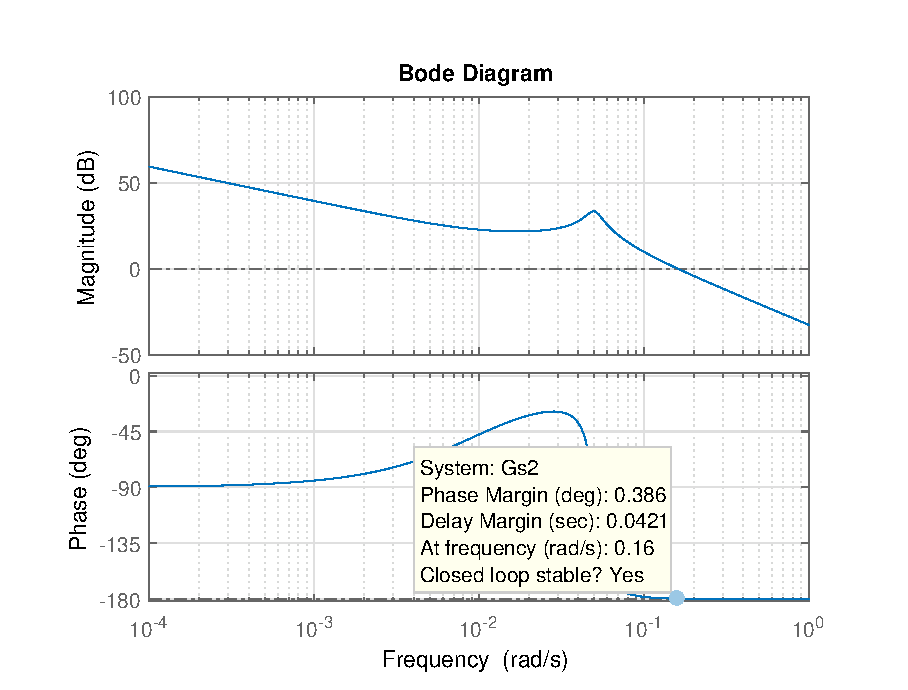
\includegraphics[width=0.5\textwidth]{./fig/Q5_B_Bode_Gained.eps}\label{fig:Q5_B_Bode_Gained}}
	\hfill
	\subfloat[Filled constant temperature lines of the 42 x 42 grid]{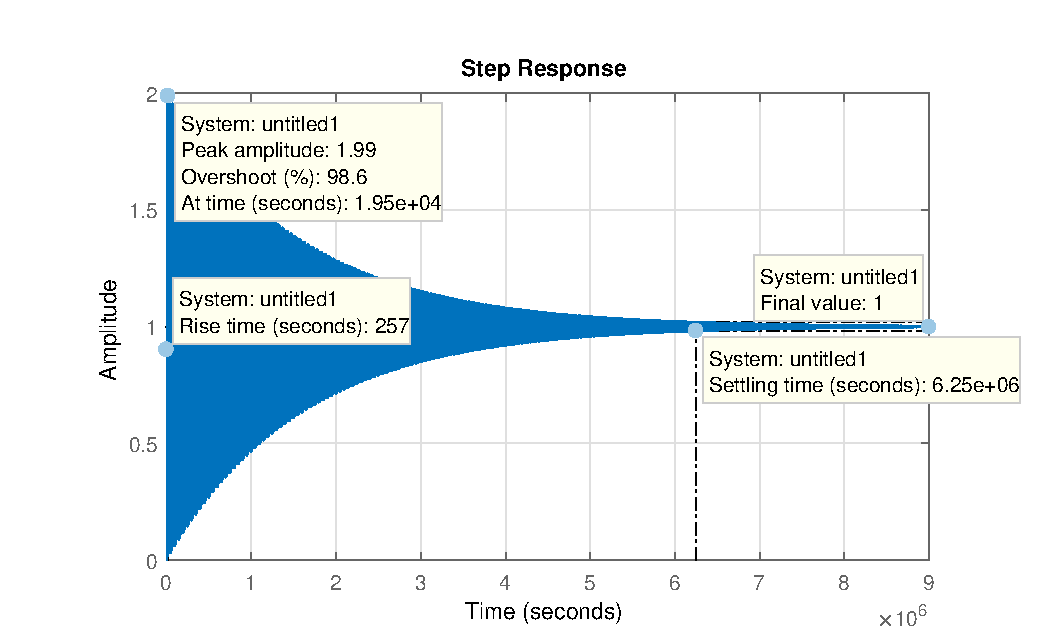
\includegraphics[width=0.5\textwidth]{./fig/Q5_G_step.eps}\label{fig:42}}
	\caption{42 x 42 grid plots}
\end{figure}

\begin{figure}[thpb]
	\centering
	
	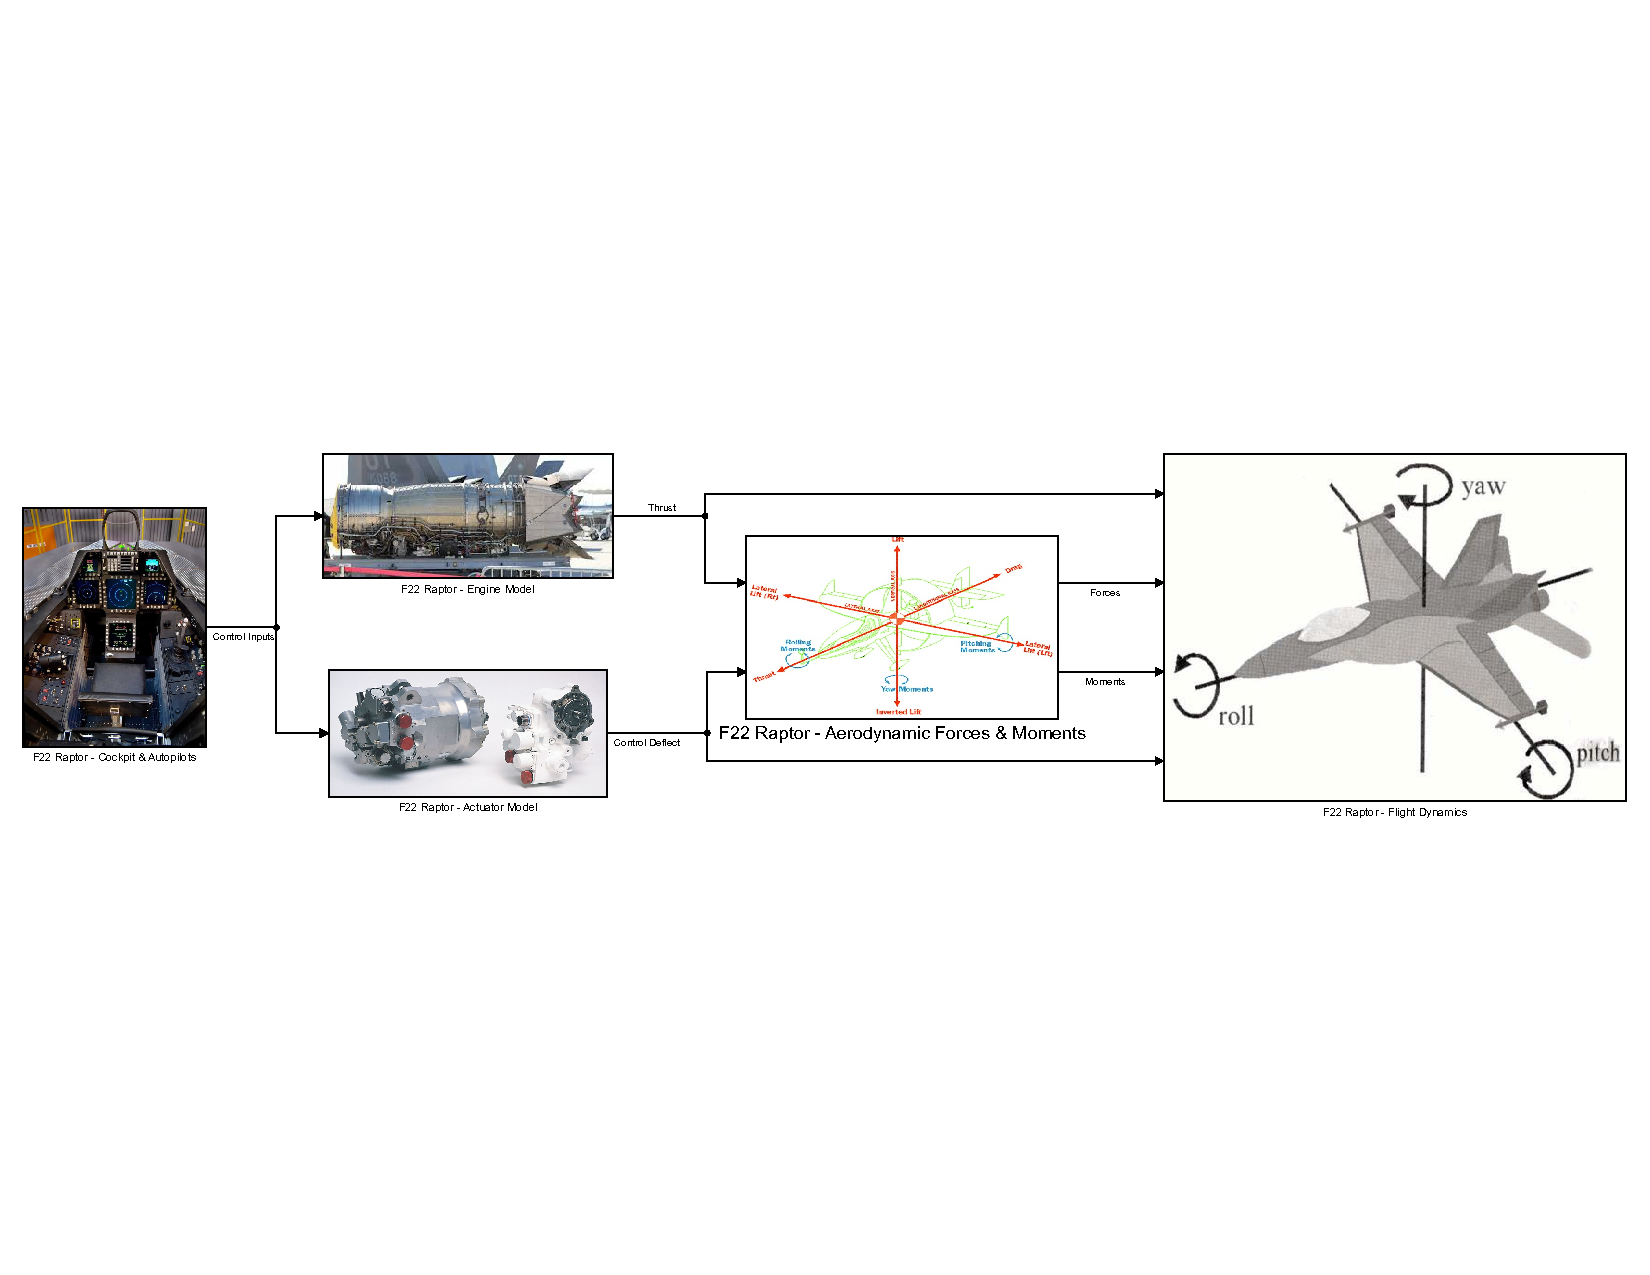
\includegraphics[trim={0 7.5cm 0 7.5cm},clip,width=\linewidth]{./fig/00_F22_Model_v2}
	
	\caption{Simulink block that has the environment model}
	\label{00F22Model} 
\end{figure}

\begin{figure}[thpb]
	\centering	
	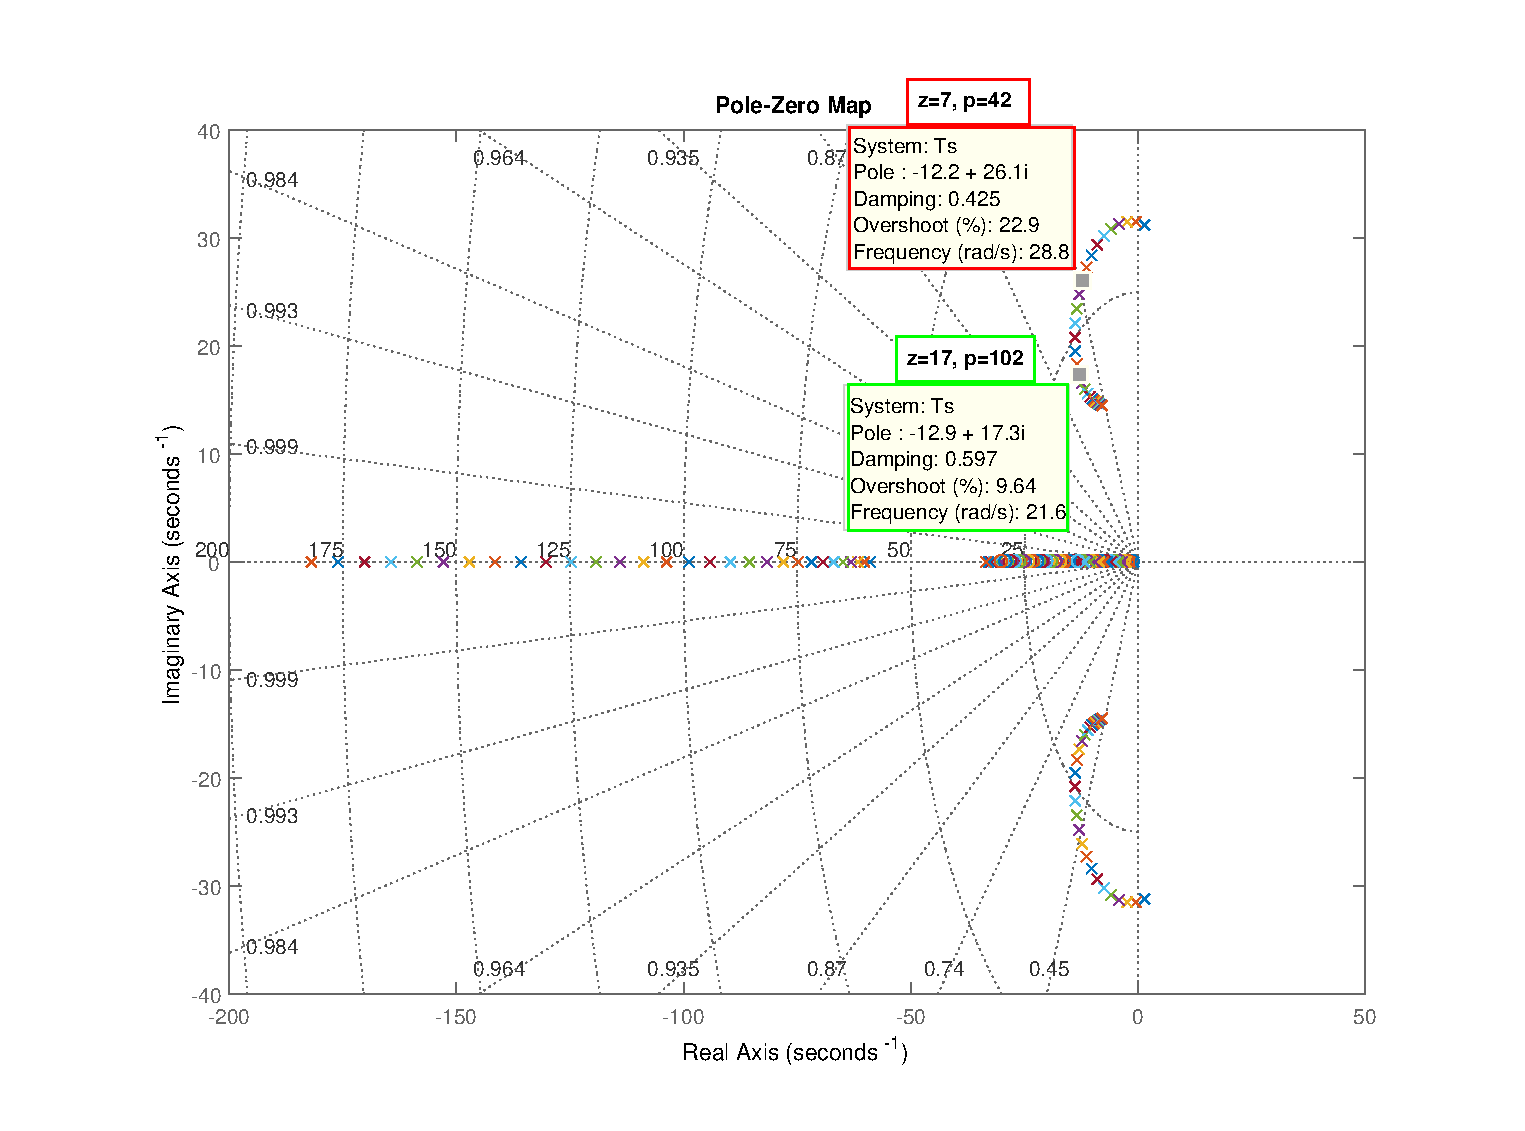
\includegraphics[width=\linewidth]{./fig/Q01_A_pzmap.eps}
	% trim={<left> <lower> <right> <upper>}
	\caption{Pole-Zero map of the closed-loop transfer function for different $z$ values}
	\label{fig:Q01_A_pzmap} 
\end{figure}


\begin{table}[thpb]
	\centering
	\caption{Permutation results}
	\label{tab:problem14}
	\begin{tabular}{|c|c|c|}
		\hline
		\textbf{Permutation}        & \textbf{Value} & \textbf{Number of the elements that are greater \& on the left} \\ \hline
		\multirow{4}{*}{\textbf{1}} & 2              & 0                                                               \\ \cline{2-3} 
		& 3              & 0                                                               \\ \cline{2-3} 
		& 4              & 0                                                               \\ \cline{2-3} 
		& 1              & 3                                                               \\ \hline
		\multirow{4}{*}{\textbf{2}} & 3              & 0                                                               \\ \cline{2-3} 
		& 4              & 0                                                               \\ \cline{2-3} 
		& 1              & 2                                                               \\ \cline{2-3} 
		& 2              & 2                                                               \\ \hline
		\multirow{5}{*}{\textbf{3}} & 5              & 0                                                               \\ \cline{2-3} 
		& 1              & 1                                                               \\ \cline{2-3} 
		& 4              & 1                                                               \\ \cline{2-3} 
		& 2              & 2                                                               \\ \cline{2-3} 
		& 3              & 2                                                               \\ \hline
	\end{tabular}
\end{table}

%----------------------------------------------------------------------------------------
%	Section 2
%----------------------------------------------------------------------------------------

\section{Sudo Part}

%----------------------------------------------------------------------------------------
%	Section 3
%----------------------------------------------------------------------------------------

\newpage
\section{Additional Part}
To cite a reference, you need to include them in your bibliography file (.bib). You can find the BibTex information from the Google Scholar or from publishers' websites \cite{franklin2015feedback}.

%----------------------------------------------------------------------------------------
%	Section 4
%----------------------------------------------------------------------------------------

\section{Sudo Part}

%----------------------------------------------------------------------------------------
%				BIBLIOGRAPHY
%----------------------------------------------------------------------------------------

\newpage
\bibliographystyle{IEEEtran}
\bibliography{Main_Bib}

%----------------------------------------------------------------------------------------
%				APPENDICES
%----------------------------------------------------------------------------------------

\newpage
\appendix

\section{MATLAB Codes}

\subsection{Initialization Code} \label{App_Int}

\lstinputlisting[caption=Plot Code]{./code/PlotMFile.m}

\end{document} 
